\chapter{Introduction}
This paper discusses two security measurements, namely Link Layer Security (LLSEC) and Datagram TLS (DTLS), within Contiki OS.

In \Cref{Chp: LLSEC} we described a LLSEC implementation in Contiki OS \textit{noncoresec} and argues that its selection of IV is not secure enough and potentially has a reset problem.

\Cref{Chp: DTLS} discusses some implementation issues of DTLS on Contiki OS.

\Cref{Chp: Appdetect} first argues that under some natures of WSN, an adversary could possibly collect more accurate timing information than usual Internet Web-application attacker. Then we described a potential sensor node application fingerprinting attack using the interaction of PING protocol and the application running on the target node.

\section{Related Work}
\cite{802154Sec} discusses some security concerns in 802.15.4.  LLSEC\cite{LLSEC} is the implementation of 802.15.4 security in Contiki.

tinydtls\cite{tinydtls} is the implementation of DTLS we used in DTLS related experiments.

\section{Experiment Setup}
All experiments are done within the Cooja simulator.

The setup is as described in \Cref{fig: Setup}.

\begin{figure}
\centering
{
	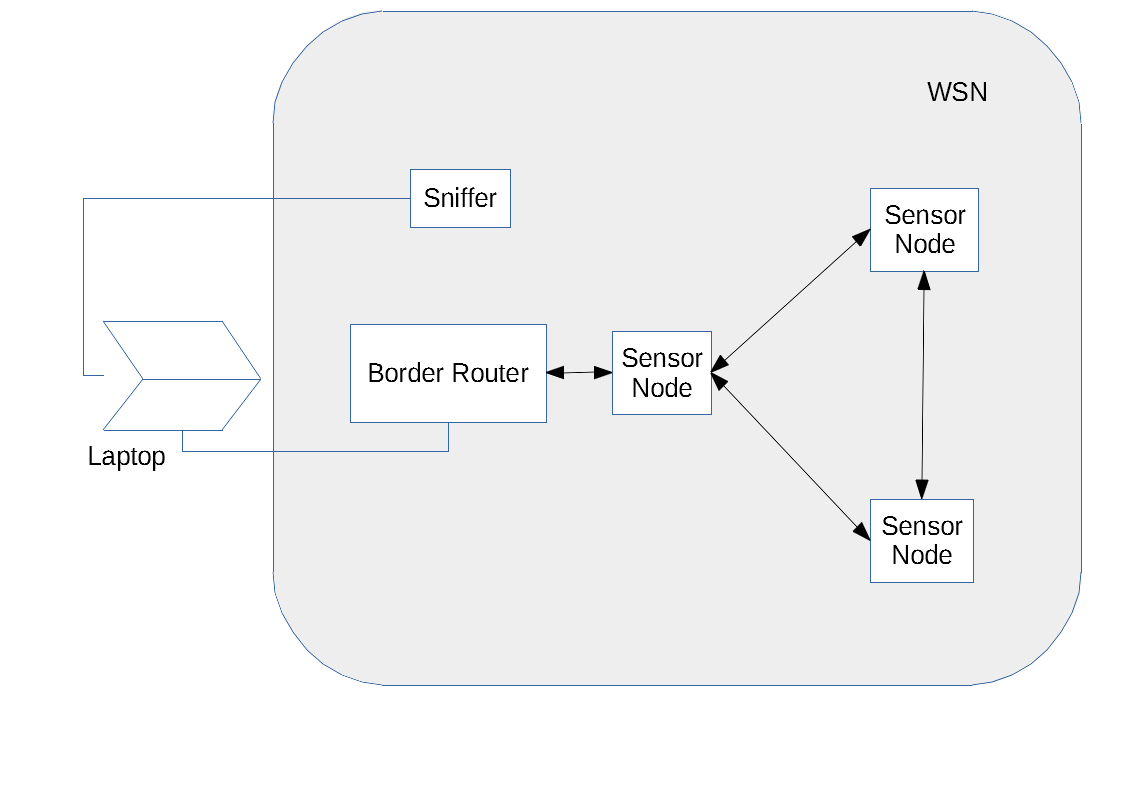
\includegraphics[width=0.7\textwidth,]{fig/setup.png}
}
\caption{Experiment setup} \label{fig: Setup}
\end{figure}

\begin{itemize}
\item{\bf Adversary} is the malicious party that tries to recover information from the encrypted traffic.
\item{\bf Border Router}, or BR, is a device that connects the adversary to the sensor network. However, \textbf{BR is not allowed when LLSEC is enabled} as the adversary does not have the key and hence cannot connect into the network. 
\item{\bf Sniffer} is a device that passively captures all traffics in the sensor network. 
\item{\bf Target} and {\bf Nodes} are sensors deployed in the sensor network. They communicates to each other through encrypted channels.
\item{\bf Sensor Network} discussed in this paper is a 6LowPAN network.
\end{itemize}

\section{Adversary Power}
The powers assumed in the experiments are considered to be practical in real life.

When LLSEC is enabled, all traffic, including RPL\footnote{Routing Procol for Low-power and Lossy Networks} messages, are encrypted; therefore no external nodes can connect to the network. The only power for the adversary is to passively sniff all the traffic.

In other cases where LLSEC is disabled, the adversary will be  enabled to join the sensor network through a BR and hence is also capable to send ICMP messages to the target(s).

\section{Types of Packets}
We simply categorise the packets into two types:
\begin{itemize}
\item {\bf Network Management Packets}: These are the packets generated by the protocols those maintains the network, such as MAC ACKs, RPL messages or ICMP messages.
\item {\bf Data Packets}: These are those packets generated by the applications running on the nodes., such as a CoAP packet.
\end{itemize}

This is only a subjective rough categorisation and may not be precise. For example an TCP data packet may also serves as an ACK, or DTLS handshake packets could fall into both categories. However, we ignore this ambiguity as it is not our focus.